\begin{abstract}
Public material attributed to channeling is distributed as interviews, creator recordings, excerpts, authored messages and publisher transcripts. Computational comparison becomes difficult when a publishing account is treated as a speaker, a repeated word as an agreed answer, or a fitted topic as an independently established category. We examine \AudioN\ retained publisher recordings through their automatic transcripts and keep \AuthoredN\ separately published texts in a distinct comparison branch. The audio material spans \AudioHours\ hours but is concentrated in nineteen Bashar-related publisher contexts and one Athina/Ashtar episode. We combine source and storage accounting, transparent TF--IDF representations, nonnegative topic construction, clustering, lexical networks, source-exclusion sensitivities and systematic model-assisted reading of selected windows. The selected two-cluster partition isolates the lone Athina recording from the nineteen Bashar-context records (cosine silhouette 0.238); stable assignment is therefore not evidence of a validated multi-practitioner taxonomy.
 The contribution is an inspectable, source-bound measurement and interpretation resource for published discourse. Speaker attribution, recognition accuracy, cross-practitioner agreement and attributed communication origins remain unverified. Human validation, authorship and institutional determinations are explicitly pending.
\end{abstract}

\section{Introduction}
An online recording is more than its title and less than a transparent record of one person's beliefs. A host may introduce a guest, read an audience question, advertise a service and frame the interpretation of what follows. A publisher may edit or redistribute an earlier recording. A machine transcript can preserve useful words while confusing a proper name, omitting a qualification or flattening different voices into a single stream. These transformations matter whenever researchers compare public accounts of unusual experiences or attributed communications.

Channeling material makes the unit problem particularly visible. Practitioners describe messages as originating from named entities, collectives or spiritual guides, while audiences encounter those descriptions through publishing platforms. The observed objects are recordings, text publications and descriptions of attribution. Determining who spoke a particular sentence, whether two recordings derive from the same session and whether two answers express the same proposition requires different evidence. None follows automatically from a shared entity label or a nearby point in a text-vector plot.

This study follows an earlier public-video index and a derivative question/answer-gist resource. Those releases established that publisher concentration, caption availability, source dependence and summarization change computational comparisons. The present work adds a distinct evidentiary layer: actual independently published audio responses, their retained automatic transcripts and separately published author text. The move from metadata to longer source material permits deeper lexical and contextual analysis. It also introduces longer-document dominance, recognition error, host and commercial language, and strong context imbalance.

The available audio is a convenience sample, not a panel of twenty mediums. Nineteen recordings concern one Bashar-related context across several publishers; one creator episode is described by its publisher as Athina Kr\'ol channeling Ashtar. Some Bashar-related recordings are interviews, promotional material or skeptical discussion. The related author's presence in a record is not a verified identity for every voice. The separate written branch contains fifteen Daniel Scranton RSS items and a Paul Selig publisher transcript framed as spiritual-Guides material. It provides a useful modality and publication comparison, with author, format and attribution confounded.

We therefore use computational breadth to expose the structure of the selected material, and source-linked readings to examine what that structure might mean. TF--IDF identifies distinctive vocabulary. Nonnegative matrix factorization (NMF) constructs reusable term components. Clustering partitions document vectors under a chosen objective. Networks retain selected similarity or co-mention relations. Their outputs can organize inspection, but they do not replace it. A large edge, a stable component or an interpretable label can still reflect introductions, advertisements, repeated publisher conventions or a topic shared by all participants.

The research questions are:
\begin{itemize}
\item \textbf{RQ1: Evidence and distribution.} What material has actually been obtained, how is it distributed across source contexts and publishers, and how does that differ from the indexed or planned YouTube collection?
\item \textbf{RQ2: Lexical construction.} Which lexical, topic and cluster structures emerge from the retained transcripts, and how sensitive are they to model choices, names, commercial vocabulary, document length and publisher composition?
\item \textbf{RQ3: Networks and overlays.} Which source and lexical relations are displayed by document, publisher-topic and claimed-group mention networks, and which interpretations are supported by their construction?
\item \textbf{RQ4: Source understanding.} What can systematic model-assisted readings and source-addressable question/answer candidates clarify, and where do speakers, prompts, answers and substantive agreement remain unresolved?
\end{itemize}

The contribution combines a source-addressable corpus description, an executed exploratory analysis with explicit perturbations, a bounded qualitative-reading and candidate-retrieval layer, and reproducible public tables, figures and manuscript sources. The analytical techniques are established baselines. The potential research value lies in making their dependencies and evidentiary boundaries inspectable in this selected domain, including negative or unstable findings. A first-in-field priority claim or a substantive claim about the origin of attributed communications is not supported by this design.

\section{Background and Related Work}
\subsection{Attributed discourse and equivalent questions}
Channeling studies differ in their elicitation conditions and units of comparison. \citet{anastasia2020qualitative} report qualitative analysis of material elicited from thirteen channels under an experimental prompt. The accessible institutional abstract and earlier reading record establish this as a precedent for contextual thematic analysis; it does not supply population theme rates for public recordings. \citet{wahbeh2023answers} distinguish numerical answer correspondence from recurring qualitative themes in scientist-supplied questions. Equivalent prompts, conditions and participant units are important precisely because a shared theme need not mean agreement on an answer.

The related prospective semantic and qualitative program is documented at different access depths in the retained register \citep{wahbeh2026semantic,wahbeh2026qualitative}. Its accessible supplementary semantic code motivates attention to concatenation and input-length handling, while unavailable publisher full text limits claims about every study procedure. Our recording-level lexical analyses do not reproduce those participant experiments.

An archival study queries separate text collections with common questions and compares AI-generated answers \citep{wahbeh2026records}. Its public supplement uses shared positive framing, making generator and prompt effects plausible contributors to resemblance. This distinction informs the present work: a source-linked answer candidate is an interpretive record for later inspection, whereas a model-generated archival answer is a new computational output. Neither is an unmediated observed answer or evidence of external truth.

Ethnographic accounts of channeling and mediumship foreground learned practice, voice, audience and interaction \citep{klinoron2014channel,tomlinson2019medium}. Our retained access to these accounts is at abstract depth. We use them to motivate contextual caution, not to claim participant ethnography. Published phrases can be analyzed without resolving the ontology of their attributed speaker, but interpretation should preserve how the material was produced and presented.

\subsection{Platform collection and source representation}
YouNiverse demonstrates why the acquisition frame, filters and missingness belong before substantive distribution claims \citep{ribeiro2021youniverse}. Its large channel/video resource has explicit thresholds and bias analysis. Our selected index does not inherit its sampling weights or population coverage. Refreshing all known IDs would improve within-index observation without establishing a complete public channel history, private/deleted coverage or a census of active practitioners.

Tube2Vec represents publishing accounts through title and description text and evaluates those representations against human tasks \citep{boesinger2024tube2vec}. It establishes account-level semantic averaging as prior practice. Here a publisher/topic overlay is a summary of selected records; topic resemblance and social position are different constructs. A graph of document similarity is not a graph of communication or influence.

\citet{chen2026digital} separate narratives, visuals and comments in religious YouTube research. Their inspected methods describe keyword discovery, explicit filtering, pilot codebooks and human review of model labels, including held-out human-coded material. The useful lesson is the separation of analytical branches and validation targets. Our automatic transcripts, lexical dictionaries and model-agent interpretations do not inherit their reliability. \citet{ota2025pathways} likewise motivate naming a network by the observed relation that creates its edges, rather than relabeling a proxy as viewing behavior or causal influence.

\subsection{Text measurement and provisional interpretation}
Text-as-data methods require validation for their intended substantive use \citep{grimmer2013text}. Topic-model research distinguishes statistical fit, interpretable terms and reliability of human meaning \citep{chang2009reading,doogan2021twaddle,hoyle2021incoherence,schroeder2025reliability}. Selecting an attractive topic count or giving components fluent names does not establish a valid ontology. The present analysis retains the candidate fits, construction rules and perturbation diagnostics alongside its selected display.

The network and topic overlays use lexical and metadata relations that can overlap within a source. A passage may mention contact, responsibility and uncertainty together, or name an astronomical system without asserting a communication from it. Source labels, keyword occurrences, model-assisted codes and verified speaker claims are therefore separate fields. Dataset documentation must also identify the language, provenance and intended use of the material \citep{bender2018statements,olteanu2019social}. The present literature synthesis reuses documented prior reading, with source-specific limits; no new systematic review or fresh full-text reading is claimed for this manuscript revision.

\section{Corpus, Acquisition, and Storage}
\subsection{From indexed leads to obtained source material}
The repository preserves a heterogeneous YouTube lead and upload index, source receipts, earlier analytical derivatives and independent publisher material. An indexed ID is evidence of a source lead, not a successful current download. Entity, practitioner, uploader, original session and publication record have distinct roles. Entity and publisher-declared civilization associations may overlap and can include unresolved or adjacent-practice labels.

Ordinary YouTube probes through the managed inherited proxy failed at CONNECT before origin TLS. The subsequent official Brave diagnostic repaired a separate browser CA-trust issue for an allowed control, then observed the same target-bound Envoy403 tunnel response. These outcomes locate a transport failure, while leaving its underlying cause undetermined. They are not evidence that YouTube served a video, denied a particular video, or classified an item as private or deleted. The new transcript study relies on independently published responses obtained from original publisher RSS enclosures and explicit author links.

\begin{table*}[t]
\centering\small
\begin{tabular}{p{0.31\textwidth}rrrr}
\toprule
Branch & Documents & Measured duration & Receipt words & Common tokens\\
\midrule
Publisher audio / unverified ASR & 20 & 22.69 h & 226,093 & 226,138\\
Authored / publisher text & 16 & not comparable & 13,575 & 13,556\\
\bottomrule
\end{tabular}
\caption{Actual analysis branches. Receipt words have different source-specific definitions and must not be pooled as a common denominator. Audio has nineteen Bashar-related source contexts and one Ashtar-attributed creator episode; written material has fifteen Daniel items and one Paul transcript.}
\label{tab:corpus}
\end{table*}
\begin{figure*}[t]
\centering
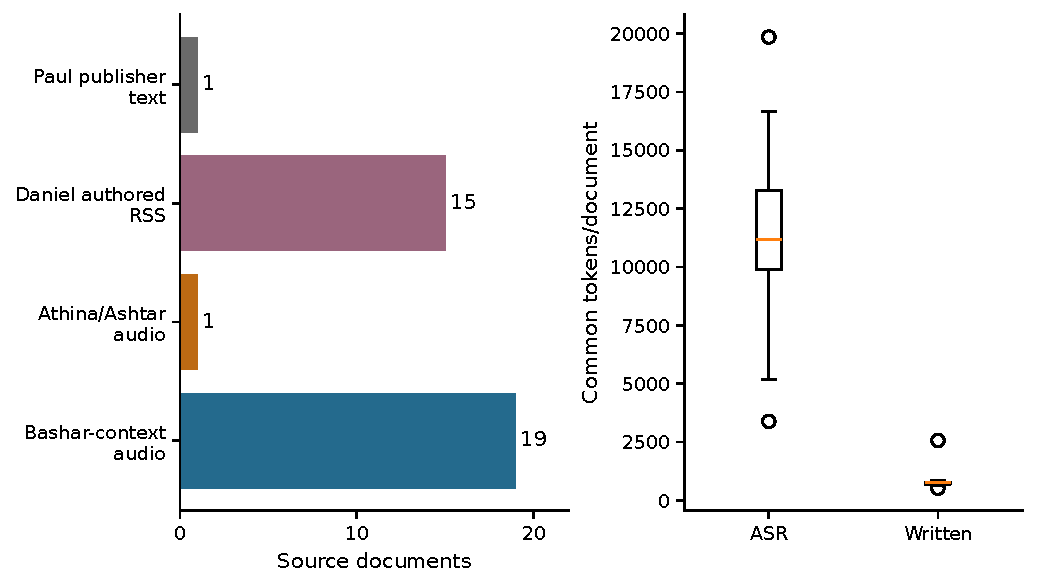
\includegraphics[width=\textwidth]{generated/figures/source-coverage.pdf}
\caption{Thirty-six source documents are two distinct modalities. Nineteen of 20 audio recordings have Bashar context; the one Ashtar-attributed creator episode is a singleton. This is not a balanced sample of mediums or civilizations. Token counts use the common analytical tokenizer, not acquisition receipt word definitions.}
\label{fig:source-coverage}
\end{figure*}


\subsection{Audio records and automatic transcripts}
Each audio source has an RSS/creator link, publication metadata, actual local bytes, hash, measured duration and acquisition outcome. Four earlier publisher responses had reviewed RSS metadata disagreements. Their accepted scope is a complete current publisher HTTP response, with original strict failures and dated amendments retained. An RSS description is not ground truth for original-session or YouTube-edition identity.

The twenty local recordings were decoded with the pinned \texttt{Systran/faster-whisper-tiny.en} model on CPU using integer-eight-bit inference, forced English, beam size one, voice activity detection and no previous-text conditioning. The retained revision is identified in the reproducibility appendix. Full decoded-audio scope distinguishes an executed complete-file pass from an explicit diagnostic clip; it does not imply that recognition captured every word. Audio, segment, transcript and source-receipt hashes bind each derivative to the recorded execution.

The ASR has no diarization or human reference transcript. Hosts, guests, skeptical commentary, advertisements and purported messages can occur in the same document. Proper names and domain-specific terms are plausible recognition-error sites. Repeated listening, word error rates and verified turn attribution are future validation tasks rather than assumptions of the present analysis.

\subsection{Separate published-text branch}
The Daniel Scranton branch contains fifteen authored RSS items from the saved feed snapshot. Its rendered bodies include any publisher titles, promotions and footers. These are fifteen documents in one author context, with several attributed labels, rather than fifteen independent practitioners. The Paul Selig branch contains a four-page publisher-issued transcript linked by the official session page. It is explicitly framed as spiritual-Guides comparison material. Correspondence between its text and an original recording is unverified.

The text branch is fitted separately for its primary lexical analysis. Its projection into the audio vocabulary is labeled as a comparison of lexical support. Differences can reflect author, source format, promotion, vocabulary support or text production. The design cannot isolate a modality effect or estimate a practitioner-group contrast from those confounded attributes.

\subsection{What storage distributions measure}
The storage ledger counts actual retained source artifacts separately from queued YouTube jobs and archive manifests. Twenty source recordings generate sixty ASR output files; text publications, PDF extraction and feed metadata are additional artifact types. Sidecars and checksums increase the number of archive objects without adding new recordings or independent observations. Byte-identical archive copies do not enlarge the research sample.

The distribution tables preserve distinct publisher-group, literal-route, practitioner-association and attributed-label views. These are overlapping metadata associations, not population counts. A publisher can host several contexts; a source can carry multiple labels. Duration, byte size and upload count answer different questions. A longer recording supplies more possible word occurrences, while a larger compressed file can reflect bitrate rather than more substantive content. Authenticated remote capacity and successful Drive storage are reported only if an actual account/transfer receipt establishes them.

\section{Analytical Methods}
\subsection{Protocol, units, and normalization}
The exploratory analysis protocol was recorded before the new calculations, after the source schema and previous work were known. This is a transparent execution order, not preregistration. A recording is the primary audio document; a publisher text is the written-branch document. Time bins and reading windows reuse documents and are not additional independent sources.

The common analysis tokenizer applies Unicode normalization, apostrophe normalization and a documented alphabetic-word rule. Lexical-rate denominators include one-letter tokens; TF--IDF excludes them. This common count differs from acquisition-receipt counts, which use whitespace words for ASR and the original extractor's rule for authored text. Counts are named rather than silently merged. Overlapping dictionary occurrences are expressed per 1,000 common analysis tokens, with equal-document summaries and pooled-token summaries retained separately.

The executed TF--IDF fit uses word unigrams and bigrams, minimum document frequency 2, maximum document frequency 0.95, and a 3,000-feature cap. The audio fit retains 3,000 features and the separate authored fit 619. The English stoplist is modified to keep negators and exclude a declared spoken-filler list. This does not make the final vector representation fully negation-preserving: the common audio unigrams no, not and never are removed by the maximum-document-frequency rule, and nor by the minimum rule; some negated bigrams can remain. The representation cannot itself establish claim stance or agreement.

NMF uses random initialization, coordinate descent and at most 1,500 iterations. Candidate component counts are 2--6, with seeds 11, 23, 47, 71 and 97. K-means uses 30 initializations for each candidate fit; the same seed set supplies stability diagnostics. The source pipeline records 457 nonoverlapping segment chunks targeting 500 tokens and 200 source-time bins. Chunks are metadata and reading aids; NMF and clustering use 20 documents, not 457 independent observations.


\subsection{TF--IDF, topic construction, and clustering}
Term frequency is sublinear, inverse document frequency is smoothed, and document vectors have L2 normalization. The audio and authored branches have separately fitted vocabularies. A cosine between their separate vector spaces would be undefined as a shared measurement. Cross-modality projection instead transforms written material using the audio-fitted vocabulary and IDF, making its support restriction explicit.

NMF approximates a nonnegative document--term matrix through nonnegative document--component and component--term factors. For display, document weights are normalized to sum to one. They are weights within the fitted representation, not fractions of speaking time, people or truth. The predeclared three-component display is accompanied by alternative component counts and seed diagnostics. Hungarian matching compares component term vectors across fits; it evaluates construction stability, not semantic validity.

K-means partitions the document TF--IDF vectors. The selected display maximizes cosine silhouette among the documented candidate counts at the reference seed. Because the display is selected using those same documents, its silhouette is an in-sample descriptive criterion. Candidate scores and adjusted-Rand seed comparisons remain visible. A two-dimensional truncated-SVD projection is a view of the audio-fitted space; distances can be distorted and axes have no independently assigned substantive meaning.

\subsection{Networks, overlays, and perturbations}
The document graph joins the union of each document's nearest lexical neighbors above the declared threshold. An edge means retained lexical similarity under that rule. Threshold sensitivity examines how graph density changes. The graph is neither a social-contact network nor an estimate of message transmission.

The claimed-group mention graph counts documents containing two dictionary families. Names such as Orion can occur in astronomical, fictional or explanatory contexts. Co-mention therefore does not verify an entity, a civilization, a speaker or coordinated origin. The publisher/topic overlay averages normalized document weights within a publisher, making source composition visible without treating the publisher as a practitioner.

Perturbations exclude explicit names, remove a predeclared commercial vocabulary, restrict segments to the central eighty percent of decoded time and omit publishing groups. These controls address measured lexical support and composition. Central-time restriction is an imperfect introduction/outro control: advertisements or hosts can remain in the middle, and attributed material can be excluded at either edge. Publisher omissions are influence diagnostics, not confidence intervals. The analysis does not report population significance, causal effects or an independently estimated number of true themes.

\subsection{Systematic model-assisted reading and candidate Q\&A}
The reading workflow selects beginning, middle, ending and query-rich windows from the available records, with deterministic source/segment locators. Query-rich selection intentionally enriches relevant passages; it is not a random or exhaustive content sample. A model agent interprets those windows using a provisional codebook. Its labels are interpretive research annotations, with support pointers and uncertainty retained. They are not independent human coding, an annotation-accuracy benchmark or a claim that every word was closely read.

Question/answer candidates preserve a source ID, transcript hash, segment/time anchors and paraphrased question and answer fields. The surrounding ASR can contain rhetorical questions, a host's question, an audience prompt, a purported response or an unanswered prompt. Candidate extraction keeps those distinctions and the unresolved speaker field visible. Recurring question wording supports retrieval and a later matched-prompt study; it does not establish semantic equivalence or answer agreement. The exact selection, code counts, candidate counts and available comparisons are generated from the executed reading artifacts below.

\section{Results}
\subsection{Obtained material and source distributions}

The audio branch contains 20 recordings from 14 publishing contexts, with median duration 66.15 minutes (range 28.05--109.92). Its actual media total is 1,691,458,021 bytes and 81,691.622 seconds. The common tokenizer yields 226,138 audio tokens and 13,556 written tokens; the original receipt totals remain 226,093 and 13,575 under their separate rules.

The current index describes 942 YouTube IDs and 362 literal routes, including 733 IDs selected under the current default collection policy. The distributions expose 180 publisher groups, 90 practitioner associations, 160 raw entity labels and 40 publisher-declared civilization labels with indexed material. Those association views overlap; none is a count of independently verified people or civilizations. Actual newly saved YouTube videos, caption tracks and bytes are all 0.

The logical storage plan contains 99 source artifacts and 1,703,635,307 bytes. The completed managed-local archive contains 200 independent copied files and 1,703,879,268 bytes, including 101 sidecar/manifest artifacts. Copies preserve the same observations. No Drive transfer, permanent external-retention guarantee or downloadable chat attachment is established by that local copy.

\subsection{Distinctive vocabulary and constructed topics}

The audio-wide mean TF--IDF vocabulary includes reality, physical, bashar, information, soul, idea, saying, change. Individual source vectors expose another layer: the Align records' top terms include protein, collagen and chocolate. Those are observable publishing/commercial vocabulary in the unsegmented transcript; treating all distinctive terms as attributed-message content would be unwarranted.

At the predeclared three-component display, seed-matched mean topic-term cosine is 0.864, with minimum 0.688. Higher stability at another component count does not identify a truer ontology. The components are labeled from their highest-weight terms in Table\ref{tab:topics}. The second component's workers/jumps/sole vocabulary is a source-inspection target, including possible recognition artifacts, rather than an independently validated conceptual category.

\begin{figure*}[t]
\centering
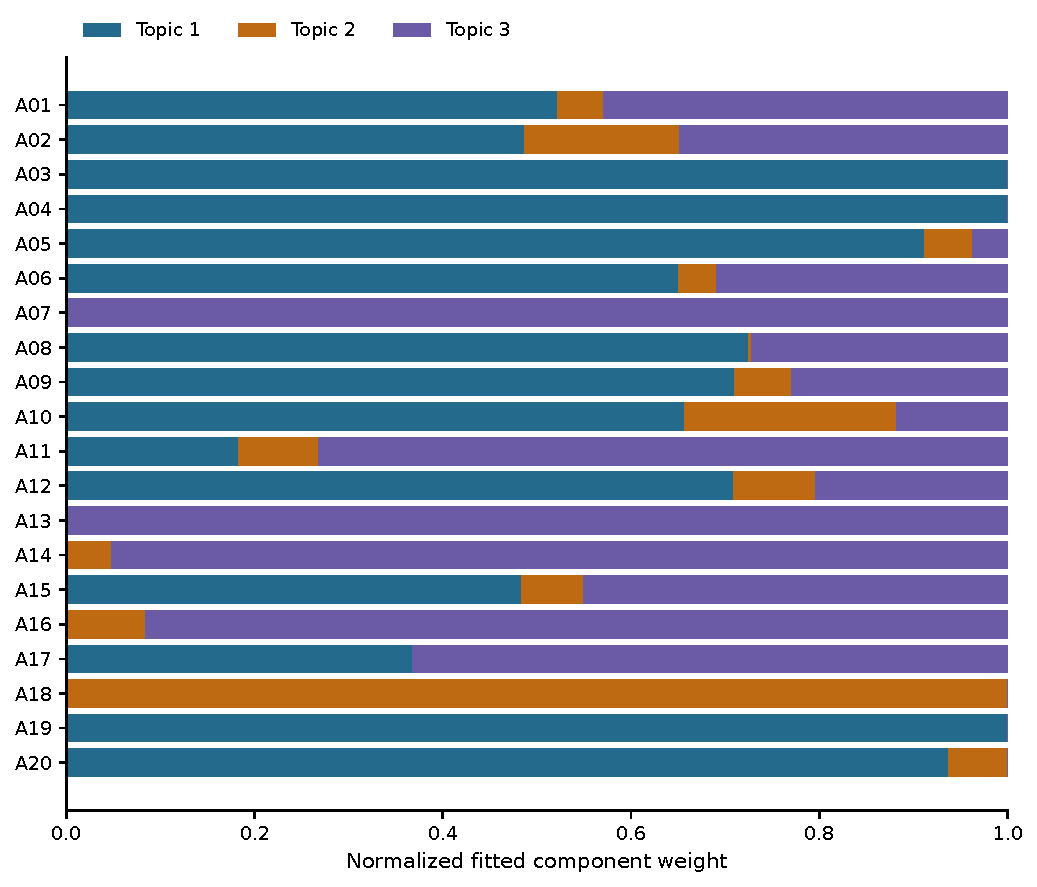
\includegraphics[width=\textwidth]{generated/figures/audio-topics.pdf}
\caption{NMF is fit to the 20 audio document vectors. Three display topics were selected prospectively for readable exploration; candidates 2--6 and seed-matched stability remain available. Weights sum to 1 per document. Top-term labels describe model components, not validated themes or distinct belief systems.}
\label{fig:audio-topics}
\end{figure*}


\begin{figure*}[t]
\centering
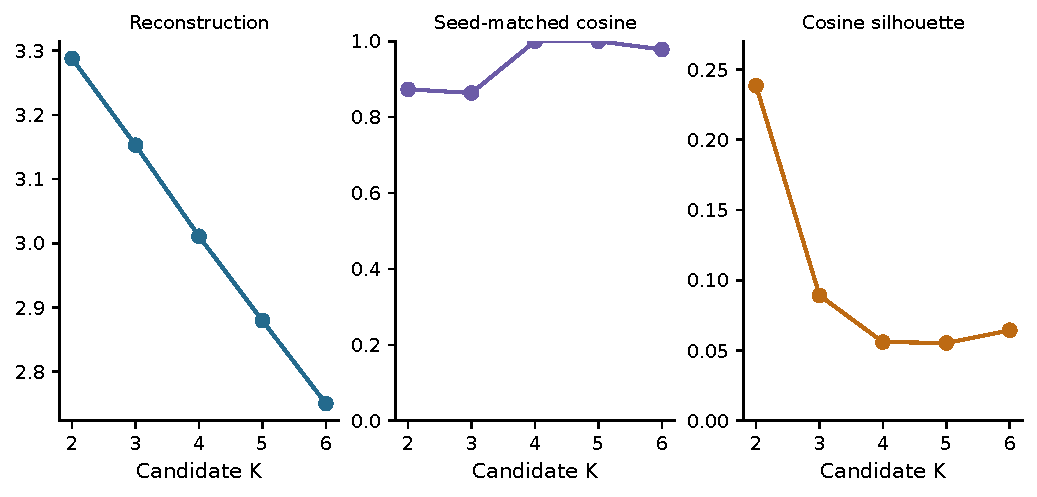
\includegraphics[width=\textwidth]{generated/figures/model-diagnostics.pdf}
\caption{NMF reconstruction decreases with model complexity and is not evidence that additional topics are substantively real. Topic stability is seed-matched term-vector cosine; KMeans selection exposes all candidate silhouettes. Neither stability nor a selected partition validates a medium or civilization ontology.}
\label{fig:model-diagnostics}
\end{figure*}


\subsection{Stable outlier partition and restricted overlays}

The selected K-means display uses K=2 and cosine silhouette 0.238. Its cluster sizes are nineteen and one: all nineteen Bashar-context recordings occupy one cluster, while the lone Athina record is the other. The cross-seed adjusted-Rand mean is 1.00. That numerical stability describes the same outlier partition. Source format, length, voice, vocabulary and context are confounded, so it cannot validate practitioner or civilization classes.

\begin{figure*}[t]
\centering
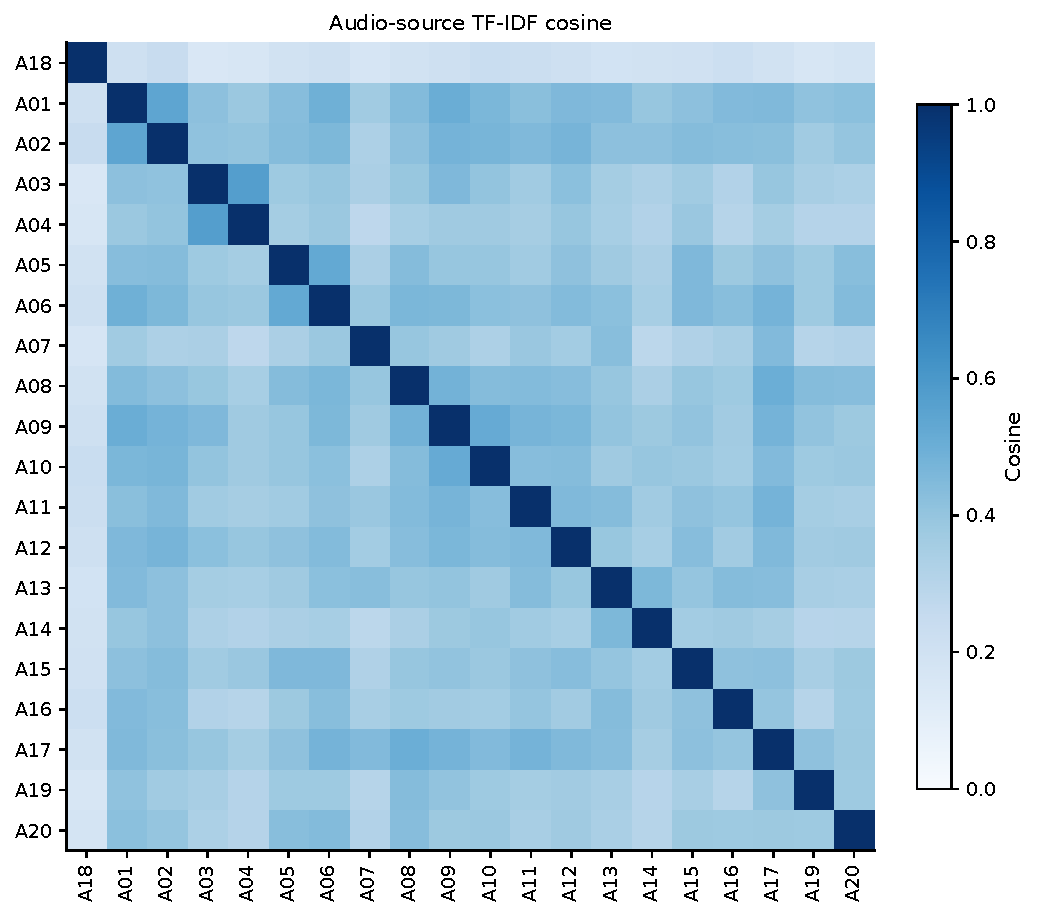
\includegraphics[width=\textwidth]{generated/figures/audio-cosine.pdf}
\caption{Cosine resemblance of 20 complete unverified ASR documents in a shared audio-only TF-IDF fit, ordered by the exploratory KMeans labels. Diagonal values are self-similarity. Short IDs join sources.json; resemblance is not semantic agreement, independent origin or a speaker comparison.}
\label{fig:audio-cosine}
\end{figure*}


\begin{figure*}[t]
\centering
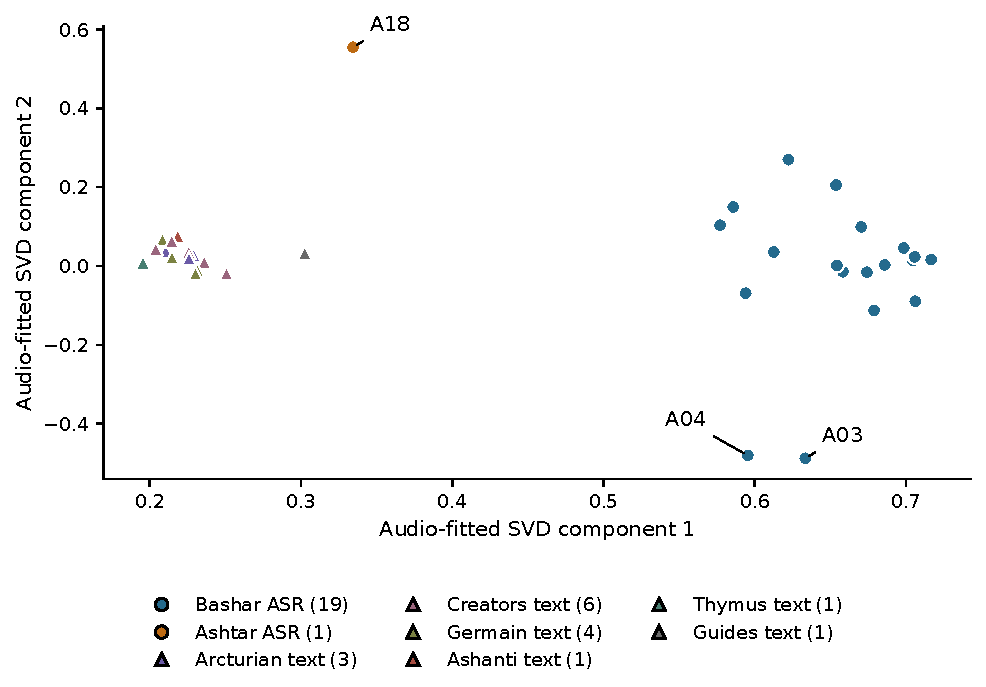
\includegraphics[width=\textwidth]{generated/figures/source-overlay.pdf}
\caption{Two-component SVD is fitted only to the 20 audio TF-IDF vectors; 16 written documents are projected through the same vocabulary and axes. Shapes distinguish modality and the short context key gives document counts. Only A03/A04 (retail-vocabulary examples) and A18 (the lone Ashtar source) are labeled to avoid crowding; all unchanged coordinates remain in analysis.json. Author, format, length and modality are confounded.}
\label{fig:source-overlay}
\end{figure*}


The two displayed SVD components explain 9.26 percent of the reported transformed-data variance. The projection is not a faithful map of every pairwise distance. Written points use the audio vocabulary and axes; they are comparison projections rather than evidence from a joint fit. The separate written NMF display is strongly shaped by author-attributed and publisher vocabulary, as its term table in the appendix shows.

The separately fitted written clustering selects K=6 by the same in-sample criterion, but its cosine silhouette is only 0.057. Cluster sizes are 3, 4, 3, 1, 4, 1. The Paul transcript and the one Thymus-labeled Daniel item are singleton clusters. This weak, source-confounded partition is not evidence for six substantive entity or civilization classes; all candidate scores are retained in the appendix.

\subsection{Lexical rates, mention graphs, and publication relations}

\begin{figure*}[t]
\centering
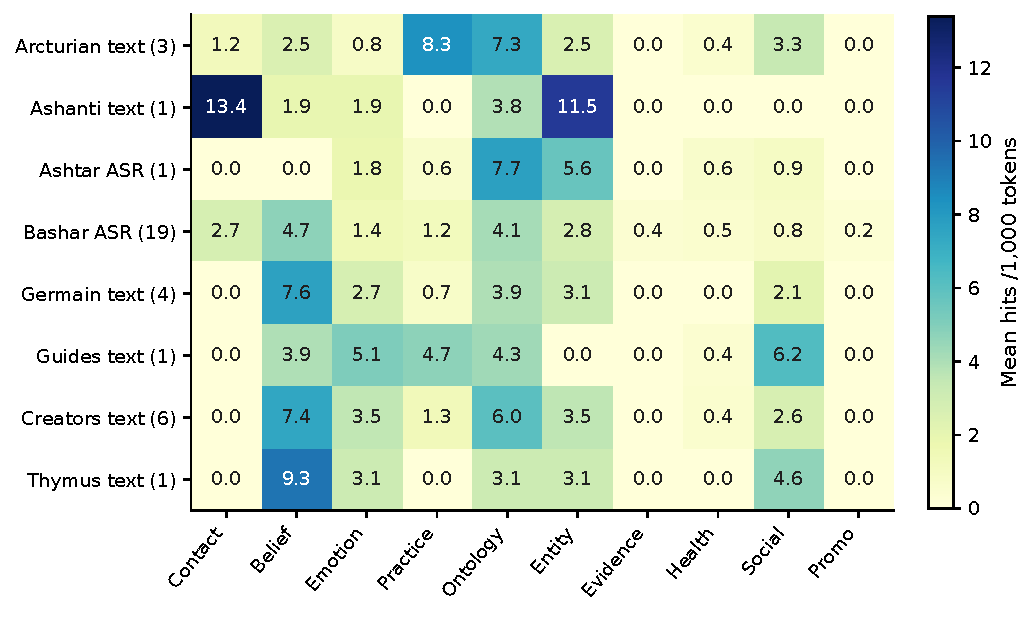
\includegraphics[width=\textwidth]{generated/figures/theme-overlay.pdf}
\caption{Overlapping predeclared keyword-family rates per 1000 common tokens, averaged equally across source documents within each labeled context. Counts are dictionary matches, not validated semantic coding. Source-attributed labels and modality are visible; singleton rows have no group-level uncertainty estimate. Promotion/footers and ASR error remain possible contributors.  Short headings follow the complete ten-family codebook order: contact/disclosure, belief/reality/agency, emotion/fear/self-worth, practice/enthusiasm/alignment, ontology/consciousness/dimensions, claimed-entity identity, epistemic validation/skepticism, health/healing, relationships/collective ethics, and commercial promotion.}
\label{fig:theme-overlay}
\end{figure*}


\begin{figure*}[t]
\centering
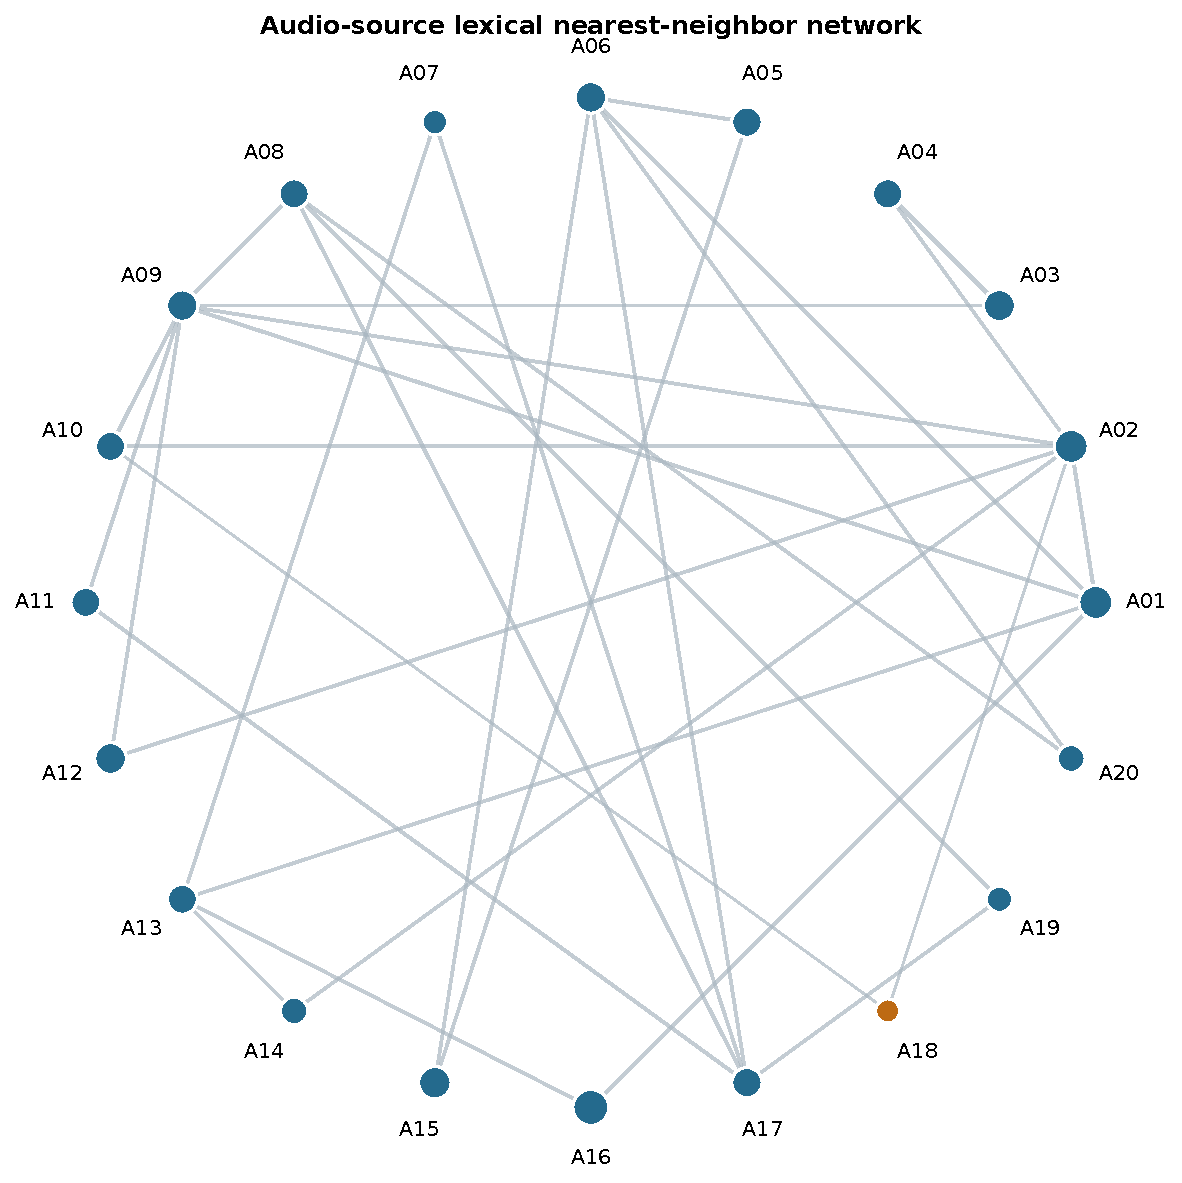
\includegraphics[width=\textwidth]{generated/figures/document-network.pdf}
\caption{Undirected union of each audio document's two nearest TF-IDF neighbors with cosine\(\geq\)0.20. Nodes are publication documents, sized by analytical token count; circular positions are purely schematic. Edges encode lexical resemblance, not social relations or independently shared ET knowledge. Threshold sensitivity is exported.}
\label{fig:document-network}
\end{figure*}


\begin{figure*}[t]
\centering
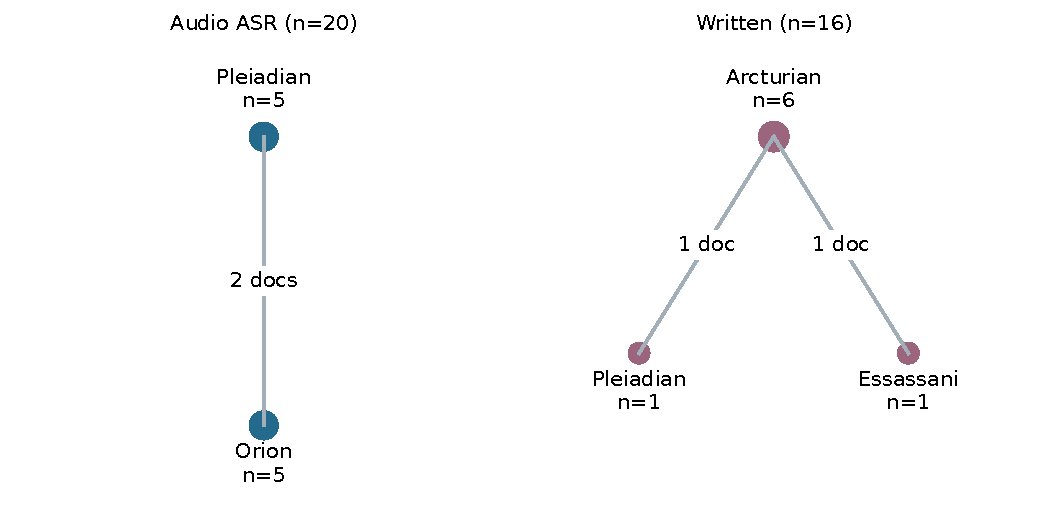
\includegraphics[width=\textwidth]{generated/figures/civilization-mentions.pdf}
\caption{Nodes are explicit claimed-civilization/star-system dictionary families and labels give documents with at least one match. Edge labels give documents mentioning both families once per pair; audio and publisher-text panels remain separate. Zero-hit families are omitted from the drawing and retained in the complete count table. Positions are schematic. Star-system/Orion mentions can concern astronomy or fiction; ASR variants are not fuzzy-corrected. Bashar and Ashtar entity names are recorded separately and are not silently mapped to a civilization.}
\label{fig:civilization-mentions}
\end{figure*}


\begin{figure*}[t]
\centering
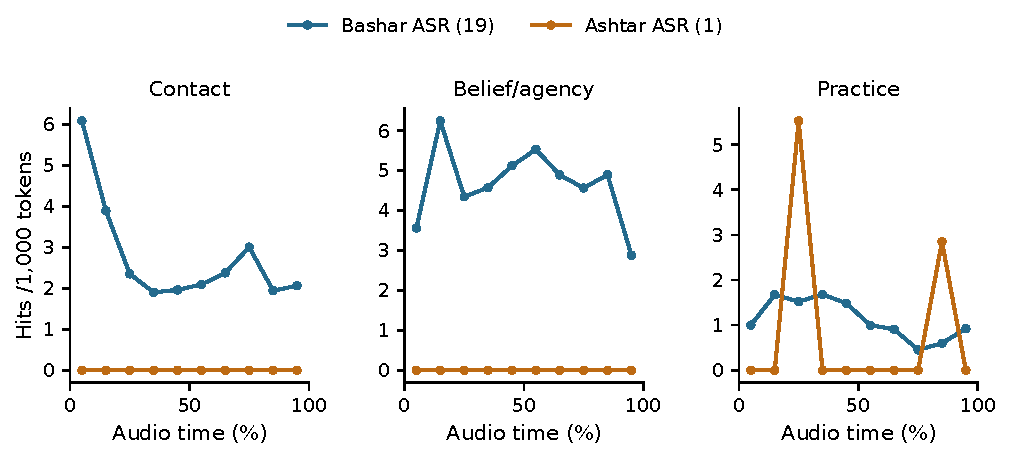
\includegraphics[width=\textwidth]{generated/figures/audio-time-profiles.pdf}
\caption{Segments are assigned by their midpoint to ten equal decoded-audio-time bins. Each bin's keyword occurrences are divided by its own common-token denominator; curves are equal-document means. The Ashtar curve represents one recording, not an estimated population trajectory. Bins are dependent and not independent observations; source intro/outro/advertising remains unsegmented.}
\label{fig:audio-time-profiles}
\end{figure*}


The displayed audio document graph retains 32 edges under its two-neighbor/threshold rule. The separate all-pair threshold diagnostic counts 190 possible reused-document pairs. Its edge counts vary from a complete graph at 0.15 to zero at 0.65; this diagnostic is not the same graph rule as the displayed top-two-neighbor union. Network density is therefore partly a construction choice, not a measured social connectivity.

The strict audio civilization/star-system dictionary returns only two nonzero families: Pleiadian / Pleiades: 5/20 documents, 6 mentions; Orion: 5/20 documents, 8 mentions. They co-occur in two documents. Missing strict matches do not establish absence of a topic, a correct ASR spelling or an attributed group. The authored branch has Arcturian/Arcturus matches in six documents, whereas three items carry the corresponding source label. This is a concrete difference between a source's attributed label and terms appearing in its body. Orion and other names remain potentially astronomical or fictional mentions.

A separately labeled post-hoc spelling sensitivity retains the strict counts and inspects unvalidated variants. Essassani / Sassani has 0 strict matches and 4 additional candidate-spelling occurrences across 4 source documents. Ashtar has 3 strict matches and 14 additional candidate-spelling occurrences across 1 source documents. These are ASR-string candidates, not audio-validated corrections or verified identity attributions; the primary dictionary graph is unchanged.

An executed synthetic control illustrates a stronger semantic limit: Following excitement is safe and Following excitement is not safe have cosine 1.00 in the actual audio-fitted space. They are purpose-built contrasting sentences, not a corpus prevalence or error-rate estimate. Lexical resemblance alone cannot test agreement or safety.

\subsection{Sensitivity and limits of simple removals}

Excluding declared proper-name tokens in the audio-ASR cohort gives pairwise-cosine rank correlation 0.998 with baseline and preserves 95 percent of nearest-neighbor choices. These are within-corpus perturbation results, not accuracy estimates.

Excluding the declared commercial vocabulary in the audio-ASR cohort gives pairwise-cosine rank correlation 0.998 with baseline and preserves 90 percent of nearest-neighbor choices. These are within-corpus perturbation results, not accuracy estimates.

Restricting ASR to the central 80 percent of audio time in the audio-ASR cohort gives pairwise-cosine rank correlation 0.945 with baseline and preserves 80 percent of nearest-neighbor choices. These are within-corpus perturbation results, not accuracy estimates.

The separate written commercial-vocabulary exclusion gives rank correlation 1.000 and preserves 100 percent of nearest-neighbor choices in that fitted written cohort. That unchanged result does not show that publisher promotion was absent or successfully removed.

Across the 14 publisher omissions, mean matched topic cosine is 0.789 and its minimum is 0.677. The original vocabulary and IDF stay fixed, so this isolates a different influence than refitting the entire pipeline. The high commercial-removal correlation is limited to its declared word list: protein, collagen and other product-specific words remain outside that list. Central-time restriction and lexical removal do not verify speaker or advertisement removal.

\subsection{Source-linked readings and question/answer candidates}

The model agent inspected 105 windows: 96 fixed windows plus 9 explicitly post-hoc or extended comparison windows. The 19,603 packet words include overlapping windows and are not unique corpus coverage. Deduplicated ASR coverage is 11,992/226,093 whitespace words (5.30 percent), across 1,112/21,197 segments. The written coverage is 6,319/13,656 whitespace words (46.27 percent). Both reading fractions use the same whitespace rule, which differs from the common analytical tokenizer and inherited written-source receipt counts. The lone Athina transcript and Paul extraction were read completely as text, while the other audio records were sampled. This asymmetric reading depth is a limitation of qualitative context comparisons. Full computational use of a transcript is not full semantic reading.

Ten provisional codes yield 142 source--code assignments supported by inspected windows. The model-assisted publisher-promotion code occurs in selected windows of 15/20 audio records and 15/16 written records. Those selected-window source-presence counts are not a population advertising rate. They also differ from a narrow commercial-word dictionary: a source can promote a book or product without matching that dictionary.

The candidate database contains 37 records in 10 provisional prompt families. Of these, 16 are analyst-constructed comparison prompts for written sources, not questions observed in an interaction. The 21 audio question-like candidates comprise 14 explicit interview-prompt candidates, one fragmentary interview prompt and six rhetorical, self-question or secondary-report candidates. They retain unsegmented question/answer turns and unknown speaker attribution. Shared family membership does not establish equivalent prompts or agreement.

The readings provide competing interpretations for numerical resemblance. A skeptical Ross/Carrie passage uses belief/reality vocabulary to criticize the guidance, whereas an Align middle window contains a retail advertisement. A Gateways reply qualifies agency rather than presenting it as literally unconstrained. The full Athina ASR separates a creator introduction, a source-framed address and closing reflection, and discusses a staged life-purpose account. Its NMF words workers, jumps and sole are interpreted in that spiritual/ASR context; the last is a potential soul homophone, not a validated correction. These paraphrases are model-agent interpretations with retained locators, not verified speaker testimony or independent human coding.

The following six case comparisons describe the actual selected material. They are interpretive findings of this window-reading exercise; differences in prompts and source formats prevent population or agreement conclusions.

\paragraph{Shared words can accompany explicit disagreement} The skeptical source restates belief/reality guidance while criticizing its repetition and ambiguity. A similarity edge to an interview therefore cannot be interpreted as agreement. Support: A16 3633.59--3693.91s.

\paragraph{Advertising and publisher framing are present in sampled source bodies} Retail advertising occurs in the temporal middle of one interview; health-service and software promotions bracket two others, and a podcast advertisement interrupts a brief organizational-role answer. Untreated document topics can therefore describe publishing infrastructure. Support: A03 2533.66--2567.74s; A01 0.00--30.16s; A02 6028.66--6062.80s; A13 1938.38--2002.82s.

\paragraph{Broad agency and future-contact themes include qualifications} One source limits changes to an earthly-life framework, another refuses to treat rapid developments as a settled forecast, and another portrays a contact forecast as conditional and potentially influenced by attention to it. These distinctions would disappear in a simple shared-keyword count. Support: A08 349.58--410.28s; A15 272.06--334.46s; A12 293.05--359.93s.

\paragraph{A singleton component needs source-level interpretation} In the Ashtar-attributed recording, workers belongs to the spiritual compound lightworkers, jumps describes claimed timeline/vibration changes, and sole occurs where surrounding text suggests a possible recognition error involving soul. These observations explain how a component can combine genuine source-specific vocabulary and transcription noise. Support: A18 113.70--138.50s; A18 348.88--455.66s; A18 846.20--876.90s.

\paragraph{A broad question family does not make answers equivalent} Contact-readiness passages address different subjects: an individual preparing for an encounter, a collective described as unready, and a selected audience described as already prepared. Their shared theme is not enough to establish agreement or contradiction. Support: A20 2676.51--2737.95s; T08 opening 250 words; T03 opening 250 words.

\paragraph{Practical guidance has different forms across the available sources} The Bashar-context exchange clarifies a general action-and-belief formula, while the complete single Ashtar comparison presents accepting, identifying and embodying a life purpose. Paul Selig and the Daniel posts offer additional spiritual framings, but these source types are not balanced evidence about separate civilizations. Support: A11 166.06--229.94s; A18 1095.10--1435.55s; T16 full text; T10 opening 250 words.

\clearpage

\section{Discussion}
\subsection{Source structure is part of the finding}
Obtaining longer source material changes the research opportunity without removing the sampling problem. A nineteen-to-one audio context imbalance cannot support a balanced comparison among mediums or attributed groups. Several publishers can add variation in framing, questioning and commercial presentation while retaining one focal context. That variation is itself meaningful for platform and discourse research, provided the document and publisher remain the named units.

The separate authored branch makes a different question possible: which vocabulary appears when these published texts are represented in a shared lexical space? It cannot attribute differences to writing versus speech alone. Source format, author, time, claimed label and promotion vary together. A useful overlay exposes those dependencies and directs inspection, rather than assigning a single cause to separation.

\subsection{Interpretable components require competing explanations}
A topic component can capture a familiar discourse theme and still be shaped by a publisher introduction, a repeated proper name or a product description. Stability across random seeds addresses optimization variability. Stability after removing names or commercial words addresses a different dependency. Stability after publisher omission addresses source composition. None tests word-recognition accuracy, prompt equivalence or participant meaning.

Likewise, a dense similarity graph can reflect common vocabulary across long documents rather than independent agreement. A group co-mention edge can be caused by an interview question listing several labels. Source-linked readings provide concrete material for examining such alternatives. Their value is greatest when they preserve counterexamples, incomplete answers and ambiguous voices instead of treating every code match as confirmation.

\subsection{Question comparison as a falsifiable next study}
The new candidate database is a route to inspectable questions, not a completed matched common-question experiment. A later design should first verify who asked and answered each prompt, identify session families and distinguish literal turns from paraphrases. It can then compare matched question classes across sufficiently varied practitioner contexts, with independent human-coded claims, uncertainty and conditions. Agreement should concern propositions and qualifications, not merely a common keyword or a shared source label.

The present results can sharpen those future decisions. Source-specific commercial vocabulary motivates speaker/promotion exclusions. Cluster or topic instability motivates held-out interpretability checks. Shared question classes motivate equivalent-prompt sampling. A candidate whose answer is absent or ambiguous is an explicit counterexample to automatic extraction completeness. The proposed analyses in the appendix state what evidence and falsifier would be needed; they are not synthetic findings.

\subsection{Contribution, reproducibility, and publication boundaries}
TF--IDF, NMF, clustering and network visualization are not new algorithms. The contribution is their source-bound integration, executed sensitivities, systematic window reading and separation of acquisition, analytical representation and substantive interpretation. More plots alone would not establish novelty or validity. An independently useful release should let a reader inspect what was obtained, how each numerical result was constructed, which source records it references and what remains unknown.

The public source bundle compiles the complete paper from frozen generated tables and figures. Recomputing the analyses additionally requires the matching lawful private source snapshots and pinned environment; full third-party speech and texts are not redistributed in Git or Pages. Source hashes support identification, not public accessibility or a redistribution license. A private organized cloud copy is a storage outcome, not an additional sample or automatically a successful third-party Drive upload.

\section{Limitations, Responsibility, and Pending Decisions}
The corpus is selected, English-focused and uneven in context and format. Original-session dependence and recording/YouTube-edition correspondence remain unresolved. Publication dates do not necessarily date the underlying communication. Metadata entity/civilization labels overlap and can reflect publisher description rather than the content or identity of a speaker.

ASR errors, unsegmented host/guest/promotional speech and word-count choices influence all downstream lexical measures. Dictionaries can miss paraphrases or count polysemous names. A topic model can emphasize artifacts, and seed stability does not establish construct validity. Graph edges and cluster assignments are constructions with reused source documents. Modality comparisons are confounded; no causal, diagnostic, population prevalence or communication-origin conclusion is justified.

The qualitative layer is model-assisted and window-based. Codebook development, selected-window enrichment and researcher expectations influence interpretation. Candidate questions and answers are paraphrases with uncertain turns and speakers; they are not a complete interview transcript or human-verified answer corpus. No new training or model-quality ranking is part of this manuscript phase.

Raw audio, full source texts, transcripts and browser profiles remain private. Published research artifacts contain source pointers, hashes, bounded vocabulary summaries, numeric outputs and interpretive paraphrases. Rights review, human authorship and affiliations, institutional determination, consent/quotation policy, independent speaker and construct validation, and any submission checklist remain \textbf{TBD}. The unmodified official AAAI/ICWSM preprint style is a writing reference. This extended living report is neither submitted nor certified as venue-compliant.

\section{Conclusion}
The obtained publisher material supports a deeper, source-addressable study of lexical structure, publication context and provisional interpretation. Its strength is the ability to connect distributions, fitted representations and selected readings back to actual retained sources while exposing the effects of analytical choices. Its central boundary is equally concrete: twenty recordings are not twenty independent mediums, a lexical network is not a communication network, and a source-linked candidate answer is not a validated proposition. The next stage is targeted human and source validation, informed by the executed sensitivities and retained ambiguities.

\section*{AI Assistance and Review}
Model agents assisted data engineering, exploratory analysis, selected-window reading, interface work and manuscript writing. The protocol specifies three iterative agent rounds covering first complete implementation, corrections and final artifact closure. Dated external review receipts identify the actual candidate hashes and completed stages.
 These reviews inspect implemented artifacts and preserve criticisms and corrections. They are not independent human peer review, participant validation or a transfer of authorship responsibility to an AI system.
